% Created by tikzDevice version 0.12.3.1 on 2023-05-03 19:54:56
% !TEX encoding = UTF-8 Unicode
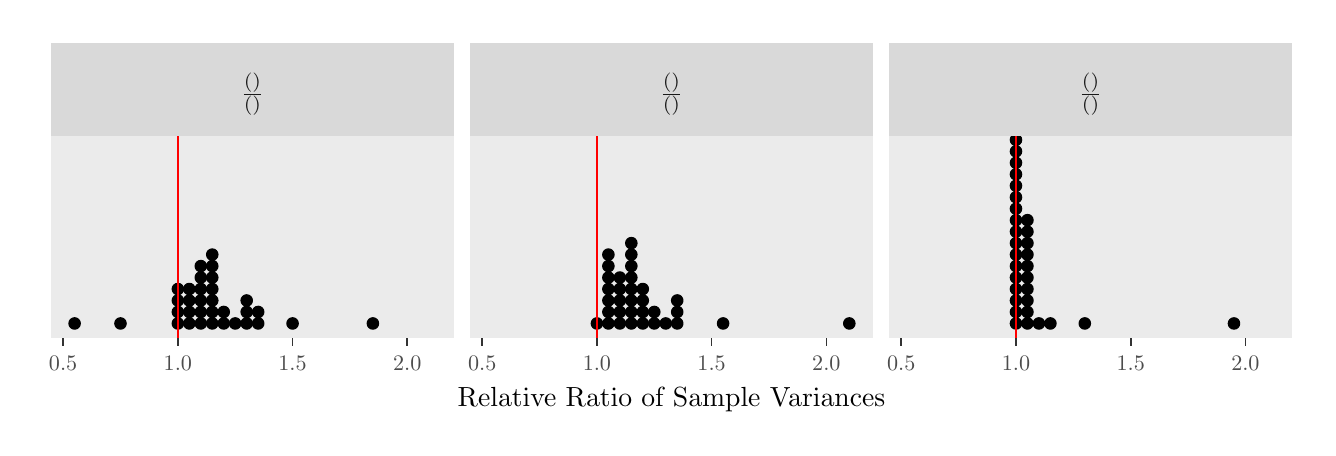
\begin{tikzpicture}[x=1pt,y=1pt]
\definecolor{fillColor}{RGB}{255,255,255}
\path[use as bounding box,fill=fillColor,fill opacity=0.00] (0,0) rectangle (462.53,144.54);
\begin{scope}
\path[clip] (  0.00,  0.00) rectangle (462.53,144.54);
\definecolor{drawColor}{RGB}{255,255,255}
\definecolor{fillColor}{RGB}{255,255,255}

\path[draw=drawColor,line width= 0.6pt,line join=round,line cap=round,fill=fillColor] (  0.00,  0.00) rectangle (462.53,144.54);
\end{scope}
\begin{scope}
\path[clip] (  8.25, 32.28) rectangle (154.18,105.24);
\definecolor{fillColor}{gray}{0.92}

\path[fill=fillColor] (  8.25, 32.28) rectangle (154.18,105.24);
\definecolor{drawColor}{RGB}{0,0,0}
\definecolor{fillColor}{RGB}{0,0,0}

\path[draw=drawColor,line width= 0.4pt,line join=round,fill=fillColor] ( 16.96, 37.66) circle (  2.07);

\path[draw=drawColor,line width= 0.4pt,line join=round,fill=fillColor] ( 33.54, 37.66) circle (  2.07);

\path[draw=drawColor,line width= 0.4pt,line join=round,fill=fillColor] ( 54.27, 37.66) circle (  2.07);

\path[draw=drawColor,line width= 0.4pt,line join=round,fill=fillColor] ( 54.27, 41.81) circle (  2.07);

\path[draw=drawColor,line width= 0.4pt,line join=round,fill=fillColor] ( 54.27, 45.96) circle (  2.07);

\path[draw=drawColor,line width= 0.4pt,line join=round,fill=fillColor] ( 54.27, 50.10) circle (  2.07);

\path[draw=drawColor,line width= 0.4pt,line join=round,fill=fillColor] ( 58.41, 37.66) circle (  2.07);

\path[draw=drawColor,line width= 0.4pt,line join=round,fill=fillColor] ( 58.41, 41.81) circle (  2.07);

\path[draw=drawColor,line width= 0.4pt,line join=round,fill=fillColor] ( 58.41, 45.96) circle (  2.07);

\path[draw=drawColor,line width= 0.4pt,line join=round,fill=fillColor] ( 58.41, 50.10) circle (  2.07);

\path[draw=drawColor,line width= 0.4pt,line join=round,fill=fillColor] ( 62.56, 37.66) circle (  2.07);

\path[draw=drawColor,line width= 0.4pt,line join=round,fill=fillColor] ( 62.56, 41.81) circle (  2.07);

\path[draw=drawColor,line width= 0.4pt,line join=round,fill=fillColor] ( 62.56, 45.96) circle (  2.07);

\path[draw=drawColor,line width= 0.4pt,line join=round,fill=fillColor] ( 62.56, 50.10) circle (  2.07);

\path[draw=drawColor,line width= 0.4pt,line join=round,fill=fillColor] ( 62.56, 54.25) circle (  2.07);

\path[draw=drawColor,line width= 0.4pt,line join=round,fill=fillColor] ( 62.56, 58.39) circle (  2.07);

\path[draw=drawColor,line width= 0.4pt,line join=round,fill=fillColor] ( 66.70, 37.66) circle (  2.07);

\path[draw=drawColor,line width= 0.4pt,line join=round,fill=fillColor] ( 66.70, 41.81) circle (  2.07);

\path[draw=drawColor,line width= 0.4pt,line join=round,fill=fillColor] ( 66.70, 45.96) circle (  2.07);

\path[draw=drawColor,line width= 0.4pt,line join=round,fill=fillColor] ( 66.70, 50.10) circle (  2.07);

\path[draw=drawColor,line width= 0.4pt,line join=round,fill=fillColor] ( 66.70, 54.25) circle (  2.07);

\path[draw=drawColor,line width= 0.4pt,line join=round,fill=fillColor] ( 66.70, 58.39) circle (  2.07);

\path[draw=drawColor,line width= 0.4pt,line join=round,fill=fillColor] ( 66.70, 62.54) circle (  2.07);

\path[draw=drawColor,line width= 0.4pt,line join=round,fill=fillColor] ( 70.85, 37.66) circle (  2.07);

\path[draw=drawColor,line width= 0.4pt,line join=round,fill=fillColor] ( 70.85, 41.81) circle (  2.07);

\path[draw=drawColor,line width= 0.4pt,line join=round,fill=fillColor] ( 74.99, 37.66) circle (  2.07);

\path[draw=drawColor,line width= 0.4pt,line join=round,fill=fillColor] ( 79.14, 37.66) circle (  2.07);

\path[draw=drawColor,line width= 0.4pt,line join=round,fill=fillColor] ( 79.14, 41.81) circle (  2.07);

\path[draw=drawColor,line width= 0.4pt,line join=round,fill=fillColor] ( 79.14, 45.96) circle (  2.07);

\path[draw=drawColor,line width= 0.4pt,line join=round,fill=fillColor] ( 83.29, 37.66) circle (  2.07);

\path[draw=drawColor,line width= 0.4pt,line join=round,fill=fillColor] ( 83.29, 41.81) circle (  2.07);

\path[draw=drawColor,line width= 0.4pt,line join=round,fill=fillColor] ( 95.72, 37.66) circle (  2.07);

\path[draw=drawColor,line width= 0.4pt,line join=round,fill=fillColor] (124.74, 37.66) circle (  2.07);
\definecolor{drawColor}{RGB}{255,0,0}

\path[draw=drawColor,line width= 0.6pt,line join=round] ( 54.27, 32.28) -- ( 54.27,105.24);
\end{scope}
\begin{scope}
\path[clip] (159.68, 32.28) rectangle (305.60,105.24);
\definecolor{fillColor}{gray}{0.92}

\path[fill=fillColor] (159.68, 32.28) rectangle (305.60,105.24);
\definecolor{drawColor}{RGB}{0,0,0}
\definecolor{fillColor}{RGB}{0,0,0}

\path[draw=drawColor,line width= 0.4pt,line join=round,fill=fillColor] (205.69, 37.66) circle (  2.07);

\path[draw=drawColor,line width= 0.4pt,line join=round,fill=fillColor] (209.84, 37.66) circle (  2.07);

\path[draw=drawColor,line width= 0.4pt,line join=round,fill=fillColor] (209.84, 41.81) circle (  2.07);

\path[draw=drawColor,line width= 0.4pt,line join=round,fill=fillColor] (209.84, 45.96) circle (  2.07);

\path[draw=drawColor,line width= 0.4pt,line join=round,fill=fillColor] (209.84, 50.10) circle (  2.07);

\path[draw=drawColor,line width= 0.4pt,line join=round,fill=fillColor] (209.84, 54.25) circle (  2.07);

\path[draw=drawColor,line width= 0.4pt,line join=round,fill=fillColor] (209.84, 58.39) circle (  2.07);

\path[draw=drawColor,line width= 0.4pt,line join=round,fill=fillColor] (209.84, 62.54) circle (  2.07);

\path[draw=drawColor,line width= 0.4pt,line join=round,fill=fillColor] (213.98, 37.66) circle (  2.07);

\path[draw=drawColor,line width= 0.4pt,line join=round,fill=fillColor] (213.98, 41.81) circle (  2.07);

\path[draw=drawColor,line width= 0.4pt,line join=round,fill=fillColor] (213.98, 45.96) circle (  2.07);

\path[draw=drawColor,line width= 0.4pt,line join=round,fill=fillColor] (213.98, 50.10) circle (  2.07);

\path[draw=drawColor,line width= 0.4pt,line join=round,fill=fillColor] (213.98, 54.25) circle (  2.07);

\path[draw=drawColor,line width= 0.4pt,line join=round,fill=fillColor] (218.13, 37.66) circle (  2.07);

\path[draw=drawColor,line width= 0.4pt,line join=round,fill=fillColor] (218.13, 41.81) circle (  2.07);

\path[draw=drawColor,line width= 0.4pt,line join=round,fill=fillColor] (218.13, 45.96) circle (  2.07);

\path[draw=drawColor,line width= 0.4pt,line join=round,fill=fillColor] (218.13, 50.10) circle (  2.07);

\path[draw=drawColor,line width= 0.4pt,line join=round,fill=fillColor] (218.13, 54.25) circle (  2.07);

\path[draw=drawColor,line width= 0.4pt,line join=round,fill=fillColor] (218.13, 58.39) circle (  2.07);

\path[draw=drawColor,line width= 0.4pt,line join=round,fill=fillColor] (218.13, 62.54) circle (  2.07);

\path[draw=drawColor,line width= 0.4pt,line join=round,fill=fillColor] (218.13, 66.68) circle (  2.07);

\path[draw=drawColor,line width= 0.4pt,line join=round,fill=fillColor] (222.27, 37.66) circle (  2.07);

\path[draw=drawColor,line width= 0.4pt,line join=round,fill=fillColor] (222.27, 41.81) circle (  2.07);

\path[draw=drawColor,line width= 0.4pt,line join=round,fill=fillColor] (222.27, 45.96) circle (  2.07);

\path[draw=drawColor,line width= 0.4pt,line join=round,fill=fillColor] (222.27, 50.10) circle (  2.07);

\path[draw=drawColor,line width= 0.4pt,line join=round,fill=fillColor] (226.42, 37.66) circle (  2.07);

\path[draw=drawColor,line width= 0.4pt,line join=round,fill=fillColor] (226.42, 41.81) circle (  2.07);

\path[draw=drawColor,line width= 0.4pt,line join=round,fill=fillColor] (230.57, 37.66) circle (  2.07);

\path[draw=drawColor,line width= 0.4pt,line join=round,fill=fillColor] (234.71, 37.66) circle (  2.07);

\path[draw=drawColor,line width= 0.4pt,line join=round,fill=fillColor] (234.71, 41.81) circle (  2.07);

\path[draw=drawColor,line width= 0.4pt,line join=round,fill=fillColor] (234.71, 45.96) circle (  2.07);

\path[draw=drawColor,line width= 0.4pt,line join=round,fill=fillColor] (251.29, 37.66) circle (  2.07);

\path[draw=drawColor,line width= 0.4pt,line join=round,fill=fillColor] (296.90, 37.66) circle (  2.07);
\definecolor{drawColor}{RGB}{255,0,0}

\path[draw=drawColor,line width= 0.6pt,line join=round] (205.69, 32.28) -- (205.69,105.24);
\end{scope}
\begin{scope}
\path[clip] (311.10, 32.28) rectangle (457.03,105.24);
\definecolor{fillColor}{gray}{0.92}

\path[fill=fillColor] (311.10, 32.28) rectangle (457.03,105.24);
\definecolor{drawColor}{RGB}{0,0,0}
\definecolor{fillColor}{RGB}{0,0,0}

\path[draw=drawColor,line width= 0.4pt,line join=round,fill=fillColor] (357.12, 37.66) circle (  2.07);

\path[draw=drawColor,line width= 0.4pt,line join=round,fill=fillColor] (357.12, 41.81) circle (  2.07);

\path[draw=drawColor,line width= 0.4pt,line join=round,fill=fillColor] (357.12, 45.96) circle (  2.07);

\path[draw=drawColor,line width= 0.4pt,line join=round,fill=fillColor] (357.12, 50.10) circle (  2.07);

\path[draw=drawColor,line width= 0.4pt,line join=round,fill=fillColor] (357.12, 54.25) circle (  2.07);

\path[draw=drawColor,line width= 0.4pt,line join=round,fill=fillColor] (357.12, 58.39) circle (  2.07);

\path[draw=drawColor,line width= 0.4pt,line join=round,fill=fillColor] (357.12, 62.54) circle (  2.07);

\path[draw=drawColor,line width= 0.4pt,line join=round,fill=fillColor] (357.12, 66.68) circle (  2.07);

\path[draw=drawColor,line width= 0.4pt,line join=round,fill=fillColor] (357.12, 70.83) circle (  2.07);

\path[draw=drawColor,line width= 0.4pt,line join=round,fill=fillColor] (357.12, 74.98) circle (  2.07);

\path[draw=drawColor,line width= 0.4pt,line join=round,fill=fillColor] (357.12, 79.12) circle (  2.07);

\path[draw=drawColor,line width= 0.4pt,line join=round,fill=fillColor] (357.12, 83.27) circle (  2.07);

\path[draw=drawColor,line width= 0.4pt,line join=round,fill=fillColor] (357.12, 87.41) circle (  2.07);

\path[draw=drawColor,line width= 0.4pt,line join=round,fill=fillColor] (357.12, 91.56) circle (  2.07);

\path[draw=drawColor,line width= 0.4pt,line join=round,fill=fillColor] (357.12, 95.70) circle (  2.07);

\path[draw=drawColor,line width= 0.4pt,line join=round,fill=fillColor] (357.12, 99.85) circle (  2.07);

\path[draw=drawColor,line width= 0.4pt,line join=round,fill=fillColor] (357.12,103.99) circle (  2.07);

\path[draw=drawColor,line width= 0.4pt,line join=round,fill=fillColor] (357.12,108.14) circle (  2.07);

\path[draw=drawColor,line width= 0.4pt,line join=round,fill=fillColor] (357.12,112.29) circle (  2.07);

\path[draw=drawColor,line width= 0.4pt,line join=round,fill=fillColor] (361.26, 37.66) circle (  2.07);

\path[draw=drawColor,line width= 0.4pt,line join=round,fill=fillColor] (361.26, 41.81) circle (  2.07);

\path[draw=drawColor,line width= 0.4pt,line join=round,fill=fillColor] (361.26, 45.96) circle (  2.07);

\path[draw=drawColor,line width= 0.4pt,line join=round,fill=fillColor] (361.26, 50.10) circle (  2.07);

\path[draw=drawColor,line width= 0.4pt,line join=round,fill=fillColor] (361.26, 54.25) circle (  2.07);

\path[draw=drawColor,line width= 0.4pt,line join=round,fill=fillColor] (361.26, 58.39) circle (  2.07);

\path[draw=drawColor,line width= 0.4pt,line join=round,fill=fillColor] (361.26, 62.54) circle (  2.07);

\path[draw=drawColor,line width= 0.4pt,line join=round,fill=fillColor] (361.26, 66.68) circle (  2.07);

\path[draw=drawColor,line width= 0.4pt,line join=round,fill=fillColor] (361.26, 70.83) circle (  2.07);

\path[draw=drawColor,line width= 0.4pt,line join=round,fill=fillColor] (361.26, 74.98) circle (  2.07);

\path[draw=drawColor,line width= 0.4pt,line join=round,fill=fillColor] (365.41, 37.66) circle (  2.07);

\path[draw=drawColor,line width= 0.4pt,line join=round,fill=fillColor] (369.56, 37.66) circle (  2.07);

\path[draw=drawColor,line width= 0.4pt,line join=round,fill=fillColor] (381.99, 37.66) circle (  2.07);

\path[draw=drawColor,line width= 0.4pt,line join=round,fill=fillColor] (435.89, 37.66) circle (  2.07);
\definecolor{drawColor}{RGB}{255,0,0}

\path[draw=drawColor,line width= 0.6pt,line join=round] (357.12, 32.28) -- (357.12,105.24);
\end{scope}
\begin{scope}
\path[clip] (  8.25,105.24) rectangle (154.18,139.04);
\definecolor{fillColor}{gray}{0.85}

\path[fill=fillColor] (  8.25,105.24) rectangle (154.18,139.04);
\definecolor{drawColor}{gray}{0.10}

\node[text=drawColor,anchor=base,inner sep=0pt, outer sep=0pt, scale=  1.00] at ( 81.21,125.21) {};

\node[text=drawColor,anchor=base,inner sep=0pt, outer sep=0pt, scale=  1.00] at ( 81.21,118.01) {$\frac{\varhat(\tsd)}{\varhat(\trebar)}$};

\node[text=drawColor,anchor=base,inner sep=0pt, outer sep=0pt, scale=  1.00] at ( 81.21,110.81) {};
\end{scope}
\begin{scope}
\path[clip] (159.68,105.24) rectangle (305.60,139.04);
\definecolor{fillColor}{gray}{0.85}

\path[fill=fillColor] (159.68,105.24) rectangle (305.60,139.04);
\definecolor{drawColor}{gray}{0.10}

\node[text=drawColor,anchor=base,inner sep=0pt, outer sep=0pt, scale=  1.00] at (232.64,125.21) {};

\node[text=drawColor,anchor=base,inner sep=0pt, outer sep=0pt, scale=  1.00] at (232.64,118.01) {$\frac{\varhat(\tsd)}{\varhat(\trc)}$};

\node[text=drawColor,anchor=base,inner sep=0pt, outer sep=0pt, scale=  1.00] at (232.64,110.81) {};
\end{scope}
\begin{scope}
\path[clip] (311.10,105.24) rectangle (457.03,139.04);
\definecolor{fillColor}{gray}{0.85}

\path[fill=fillColor] (311.10,105.24) rectangle (457.03,139.04);
\definecolor{drawColor}{gray}{0.10}

\node[text=drawColor,anchor=base,inner sep=0pt, outer sep=0pt, scale=  1.00] at (384.06,125.21) {};

\node[text=drawColor,anchor=base,inner sep=0pt, outer sep=0pt, scale=  1.00] at (384.06,118.01) {$\frac{\varhat(\trebar)}{\varhat(\trc)}$};

\node[text=drawColor,anchor=base,inner sep=0pt, outer sep=0pt, scale=  1.00] at (384.06,110.81) {};
\end{scope}
\begin{scope}
\path[clip] (  0.00,  0.00) rectangle (462.53,144.54);
\definecolor{drawColor}{gray}{0.20}

\path[draw=drawColor,line width= 0.6pt,line join=round] ( 12.81, 29.53) --
	( 12.81, 32.28);

\path[draw=drawColor,line width= 0.6pt,line join=round] ( 54.27, 29.53) --
	( 54.27, 32.28);

\path[draw=drawColor,line width= 0.6pt,line join=round] ( 95.72, 29.53) --
	( 95.72, 32.28);

\path[draw=drawColor,line width= 0.6pt,line join=round] (137.18, 29.53) --
	(137.18, 32.28);
\end{scope}
\begin{scope}
\path[clip] (  0.00,  0.00) rectangle (462.53,144.54);
\definecolor{drawColor}{gray}{0.30}

\node[text=drawColor,anchor=base,inner sep=0pt, outer sep=0pt, scale=  0.80] at ( 12.81, 20.71) {0.5};

\node[text=drawColor,anchor=base,inner sep=0pt, outer sep=0pt, scale=  0.80] at ( 54.27, 20.71) {1.0};

\node[text=drawColor,anchor=base,inner sep=0pt, outer sep=0pt, scale=  0.80] at ( 95.72, 20.71) {1.5};

\node[text=drawColor,anchor=base,inner sep=0pt, outer sep=0pt, scale=  0.80] at (137.18, 20.71) {2.0};
\end{scope}
\begin{scope}
\path[clip] (  0.00,  0.00) rectangle (462.53,144.54);
\definecolor{drawColor}{gray}{0.20}

\path[draw=drawColor,line width= 0.6pt,line join=round] (164.24, 29.53) --
	(164.24, 32.28);

\path[draw=drawColor,line width= 0.6pt,line join=round] (205.69, 29.53) --
	(205.69, 32.28);

\path[draw=drawColor,line width= 0.6pt,line join=round] (247.15, 29.53) --
	(247.15, 32.28);

\path[draw=drawColor,line width= 0.6pt,line join=round] (288.60, 29.53) --
	(288.60, 32.28);
\end{scope}
\begin{scope}
\path[clip] (  0.00,  0.00) rectangle (462.53,144.54);
\definecolor{drawColor}{gray}{0.30}

\node[text=drawColor,anchor=base,inner sep=0pt, outer sep=0pt, scale=  0.80] at (164.24, 20.71) {0.5};

\node[text=drawColor,anchor=base,inner sep=0pt, outer sep=0pt, scale=  0.80] at (205.69, 20.71) {1.0};

\node[text=drawColor,anchor=base,inner sep=0pt, outer sep=0pt, scale=  0.80] at (247.15, 20.71) {1.5};

\node[text=drawColor,anchor=base,inner sep=0pt, outer sep=0pt, scale=  0.80] at (288.60, 20.71) {2.0};
\end{scope}
\begin{scope}
\path[clip] (  0.00,  0.00) rectangle (462.53,144.54);
\definecolor{drawColor}{gray}{0.20}

\path[draw=drawColor,line width= 0.6pt,line join=round] (315.66, 29.53) --
	(315.66, 32.28);

\path[draw=drawColor,line width= 0.6pt,line join=round] (357.12, 29.53) --
	(357.12, 32.28);

\path[draw=drawColor,line width= 0.6pt,line join=round] (398.57, 29.53) --
	(398.57, 32.28);

\path[draw=drawColor,line width= 0.6pt,line join=round] (440.03, 29.53) --
	(440.03, 32.28);
\end{scope}
\begin{scope}
\path[clip] (  0.00,  0.00) rectangle (462.53,144.54);
\definecolor{drawColor}{gray}{0.30}

\node[text=drawColor,anchor=base,inner sep=0pt, outer sep=0pt, scale=  0.80] at (315.66, 20.71) {0.5};

\node[text=drawColor,anchor=base,inner sep=0pt, outer sep=0pt, scale=  0.80] at (357.12, 20.71) {1.0};

\node[text=drawColor,anchor=base,inner sep=0pt, outer sep=0pt, scale=  0.80] at (398.57, 20.71) {1.5};

\node[text=drawColor,anchor=base,inner sep=0pt, outer sep=0pt, scale=  0.80] at (440.03, 20.71) {2.0};
\end{scope}
\begin{scope}
\path[clip] (  0.00,  0.00) rectangle (462.53,144.54);
\definecolor{drawColor}{RGB}{0,0,0}

\node[text=drawColor,anchor=base,inner sep=0pt, outer sep=0pt, scale=  1.00] at (232.64,  7.83) {Relative Ratio of Sample Variances};
\end{scope}
\end{tikzpicture}
